\section{A funkciók megvalósítása}

Az alábbiakban a szakdolgozat részeit képzeő általam megvalósított funkciókhoz
létrehozott osztályok kerülnek bemutatásra, továbbá az alkalmazás
állapotobjektumának az adott funkciók működéséhez szükséges részei és az azok
módosítására szolgáló akciók.

\subsection{Hőtérképes megjelenítés}

\noindent Az ehhez megvalósított osztályok:
\begin{itemize}

\item\subsubsection{HeatmapLayerSettingsPresentation}
A hőtérkép réteg beállításait tartalmazó komponens.
Itt adhatóak meg az aktuális réteg úgymond "feliratkozásai", tehát, hogy melyik
eszköz melyik csatornáján érkező adatok megjelenítését végezze.

Ezek a csatornák a következőképpen működnek. A szerverben minden drónhoz (UAV)
lehetnek rendelve eszközök (device), amiken belül akár több különböző csatorna
(channel) is elérhetővé tehető. Amennyiben egy ilyen "UAV/device/channel"
elérési útra feliratkozik egy kliens, akkor minden alkalommal, amikor elérhetővé
válik egy újabb mérési eredmény, arról értesítést kap a szervertől egy olyan
objektum formájában, ami tartalmazzaa mérés eredményét, valamint a hozzá
tartozó időbélyeget és pozíciót.

Beállítható továbbá a jelölők közötti távolság, hogy rácspontokon kerüljenek-e
elhelyezésre, vagy pedig minél közelebb a mérés helyéhez, valamint a skála
végpontjai, hogy automatikusan skálázódjon-e újabb extremális értékek
érkezésekor, illetve hogy lineáris vagy pedig logaritmikus legyen.

\item\subsubsection{HeatmapVectorSource}
Az \verb|ol-react| csomag által biztosított \verb|source.Vector| osztályból
származtatott osztály, amely a hőtérképen megjelenő színes jelölők
létrehozásáért és frissítéséért felelős.
A drónokról érkező üzenetek feldolgozása és az adatok \verb|localStorage|-be
történő szinkronizálása is ebben az objektumban történik, így újratöltéskor nem
vesznek el az eddigi mérés eredményei.

\item\subsubsection{HeatmapLayerPresentation}
A hőtérképet megjelenítő réteg. Kirajzolja a \verb|HeatmapVectorSource|-ból
származó jelölőket, a térkép sarkába pedig egy színátmenetes skálát az
értékekhez.

\end{itemize}
\noindent A háttérben lévő állapot ehhez tartozó részlete:
\begin{itemize}

  \item \textbf{state.layers.<heatmap\_layer\_name>.parameters}

  Akár több heatmap réteg is létezhet egyszerre, ezek mindegyikéhez tarozik egy
  objektum az állapotban, ami a következő paramétereket tárolja:

  \begin{itemize}
  \item \textit{subscriptions}:
    A feliratkozások (UAV/eszköz/csatorna) listája.
    (Alapértelmezett értéke: [], tehát egy üres lista)
  \item \textit{minHue}:
    A színskála alacsony végéhez tartozó kezdeti szín.
    (Alapértelmezett értéke: 100, tehát zöld szín.)
  \item \textit{maxHue}:
    A színskála magas végéhez tartozó kezdeti szín.
    (Alapértelmezett értéke: 0, tehát piros szín.)
  \item \textit{threshold}:
    Egy küszöbérték, ami alatt a mérési pontok jelentéktelennek tekinthetőek,
    fehér színnel jelennek meg.
    (Alapértelmezett értéke: 0.)
  \item \textit{coloringFunction}:
    A színezéshez felhasznált függvény azonosítója)
    (Alapértelmezett értéke: 'linear', tehát egyenletes színezés.)
  \item \textit{minValue}:
    A skála alacsony végéhez tartozó mérési érték.
    (Alapértelmezett értéke: 0.)
  \item \textit{maxValue}:
    A skála magas végéhez tartozó mérési érték.
    (Alapértelmezett értéke: 0.)
  \item \textit{autoScale}:
    A réteg azon paramétere, amely azt befolyásolja, hogy új szélsőséges adat
    érkezésekor módosuljon-e automatikusan a megfelelő irányhoz tartozó határ.
    (Alapértelmezett értéke: true, tehát a funkció be van kapcsolva.)
  \item \textit{maxPoints}:
    A réteg által tárolni kívánt pontok maximális száma.
    (Alapértelmezett értéke: 1000.)
  \item \textit{unit}:
    A réteg által megfigyelt eszköz által mért mennyiségek mértékegysége.
    A skálához tartozó jelölők megjelenítéséhez van rá szükség.
    (Alapértelmezett értéke: ''.)
  \item \textit{minDistance}:
    A réteg által kijelzett pontok közötti minimális távolság méterben mérve.
    (Alapértelmezett értéke: 5.)
  \item \textit{snapToGrid}:
    A réteg azon paramétere, amely azt befolyásolja, hogy a megjelenített pontok
    egy fix rácsra legyenek-e igazítva.
    (Alapértelmezett értéke: false, tehát a funkció ki van kapcsolva.)
  \end{itemize}

\end{itemize}


\subsection{Térkép állapotainak (pozíció, forgatás, nagyítás) tárolása és betöltése}

\noindent Az ehhez megvalósított osztályok:
\begin{itemize}

\item\subsubsection{MapReferenceRequestHandler}
A központi OpenLayers térkép példány objektumhoz történő közvetlen hozzáférésre
a programban több helyen is szükség van. Ez a komponens szolgál az ilyen jellegű
igények kielégítésére oly módon, hogy feliratkozik a központi
\verb|mapReferenceRequestSignal| jelzésre, és minden ezen keresztüli üzenetben
érkező callback függvényt meghív a térkép objektum referenciájával
paraméterként. Ehhez a referenciához úgy fér hozzá, hogy a térkép React
komponensének leszármazottjaként van elhelyezve a komponensek fájában, így a
kontextus objektumából el tudja érni.

\item\subsubsection{MapViewManager}
A központi OpenLayers térkép példány nézeti objektumának kezelésére szolgáló
osztály. Folyamatosan tárolja az aktuális pozíciót, elfordulást és nagyítást,
valamint feliratkozik az ezekhez tartozó OpenLayers API által nyújtott
eseményekre, hogy mindig frissíteni tudja az értékeket, ha szükséges, így ezek
az adatok bármikor lekérdezhetőek belőle. Ezen felül képes a térkép nézeti
paraméterének animált módosításaira is például egy elmentett állapot
visszatöltéséhez, vagy mondjuk adott drónhoz ugráshoz.

\item\subsubsection{SavedLocationEditorDialog}
Az elmentett térképállapotok szerkesztésére szolgáló dialógusablak, amelyben
szerkeszthető egy adott bejegyzés neve, középpontjának szélességi és hosszúsági
foka, elforgatási szöge és nagyítási mértéke, illetve törölhető is a bejegyzés.

\item\subsubsection{SavedLocationList}
Az elmentett térképállapotok felsorolására szolgáló lista, melynek első eleme
állandóan a jelenlegi állapotot tartalmazza, és arra történő kattintással az
aktuális adatok felvehetőek a listába. A lista egyéb elemeire kattintva az
azokhoz tartozó paraméterek által jelölt állapotba ugrik a térkép, a mellettük
lévő fogaskerékre kattintva pedig az adott állapot szerkesztését és törtését
lehetővé tevő dialógusablak nyílik meg.

\end{itemize}
\noindent A háttérben lévő állapot ehhez tartozó részlete:
\begin{itemize}

  \item \textbf{state.savedLocations}

  Az eltárolt pozíciók adatait (név, középpont, nagyítás, elforgatás)
  tartalmazó objektumokból álló állapot.

  \textit{Módosítására szolgáló műveletek:}

  \begin{itemize}
    \item UPDATE\_SAVED\_LOCATION \\
      Meglévő elmentett pozíció módosítása, vagy ha a paraméterként kapott
      pozíció az éppen aktuális pozíció, akkor új bejegyzés létrehozása.

    \item DELETE\_SAVED\_LOCATION \\
      Egy előzőleg elmentett pozíció törlése annak azonosítója alapján.
  \end{itemize}

\end{itemize}


\subsection{Objektumok betöltése GeoJSON formátumból}

\noindent Az ehhez megvalósított osztályok:
\begin{itemize}

\item\subsubsection{GeoJSONLayerSettingsPresentation}
A GeoJSON formátumban tárolt geometriák megjelenítésére szolgáló réteg
beállításait tartalmazó osztály. Megadható a rétegre betöltött objektumok
kitöltésének és körvonalának színe, valamint itt található egy szövegdoboz is,
amibe a kívánt GeoJSON adatokat kell beilleszteni, majd pedig az alatta lévő
gomb segítségével validálni és importálni a térképre.

\item\subsubsection{GeoJSONVectorSource}
Az \verb|ol-react| csomag által biztosított \verb|source.Vector| osztályból
származtatott osztály, amely a GeoJSON rétegen megjelenő geometriák stílusának
beállításáért és az OpenLayers beépített GeoJSON olvasójának segítségével
történő előállításáért felelős a \verb|GeoJSONLayerPresentation| osztály
számára.

\item\subsubsection{GeoJSONLayerPresentation}
Megjeleníti a \verb|GeoJSONVectorSource| által előállított geometriákat a
térképen.

\end{itemize}
\noindent A háttérben lévő állapot ehhez tartozó részlete:
\begin{itemize}

  \item \textbf{state.layers.<geojson\_layer\_name>.parameters}

  Akár több heatmap réteg is létezhet egyszerre, ezek mindegyikéhez tarozik egy
  objektum az állapotban, ami a következő paramétereket tárolja:

  \begin{itemize}
  \item \textit{data}:
    Az megjeleníteni kívánt geometriákat leíró adatokat tartalmazó JSON
    objektum.
    (Alapértelmezett értéke: {}.)
  \item \textit{strokeColor}:
    A megjeleníette geometriák körvonalának színe.
    (Alapértelmezett értéke: {r: 85, g: 85, b: 225, alpha: 1}, tehát sötét
    átlátszatlan kék.)
  \item \textit{strokeWidth}:
    A megjelenített geometriák körvonalának szélessége pixelekben mérgve.
    (Alapértelmezett értéke: 2.)
  \item \textit{fillColor}:
    A megjeleníette geometriák kitöltésének színe.
    (Alapértelmezett értéke: {r: 170, g: 170, b: 225, alpha: 0.5}, tehát világos
    félig átlátszó kék.)
  \end{itemize}

\end{itemize}

\subsection{Parancsok kiadása drónoknak menüsorról és jobb egérgombra felugró ablakból}

\noindent Az ehhez megvalósított osztályok:
\begin{itemize}

% \item\subsubsection{MapToolbar}
% A térképpel kapcsolatos eszközöket tartalmazó eszköztár. Különböző módok
% választhatóak rajta, amik az egérrel végrehajtható akciókat befolyásolják. Az
% elérhető módok: kijelölés, mozgatás, nagyítás. Található még rajta továbbá egy
% szövegdoboz, ami a térkép elfordulását mutatja fokokban, és a felhasználó által
% is átírható egy kívánt szög beállításának céljából. Ezeken felül még két gombot
% tartalmaz, egyet az északi orientáció visszaállítására, egyet pedig a térkép oly
% módon történő pozicionálására, hogy az összes jelenleg látható objektum
% beleférjen a képbe.

\item\subsubsection{UAVToolbar}
A drónokkal kapcsolatos eszközöket tartalmazó eszköztár. Kezdeményezhető róla
parancs kiadása a jelenleg kijelölt drónoknak. (Felszállás, leszállás,
visszatérés a kiindulópontra, kikapcsolás.) Ezen felül megnyitható róla a
tetszőleges üzenet küldésére szolgáló dialógusablak is. (Ez a lehetőség a
szoftver jelenlegi állapotában nem bír valódi funkcionalitással, a jövőre nézve
lesz jelentőssége.)

\item\subsubsection{ContextMenu}
A térkép egy üres részén vagy egy drón fölött kezdeményezett jobb egérgomb
esemény következtében megjelenő helyi menüt megvalósító osztály. A drónoknak
kiadható utasításokat tartalmazza. (Felszállás, leszállás, visszatérés a
kiindulópontra, kikapcsolás.)

\end{itemize}

\noindent A háttérben lévő állapot ehhez tartozó részlete:
\begin{itemize}

  \item \textbf{state.map.selection}

  Az aktuálisan kiejlölés alatt álló drónok listája. Egy parancs kiadásakor a
  megfelelő üzenet az ebben a listában szereplő azonosítóval rendelkező drónok
  számára kerül kiküldésre.

\end{itemize}

\subsection{Állapotüzenetek (információk, figyelmeztetések, hibák) kijelzésére alkalmas panel}

\noindent Az ehhez megvalósított osztályok:
\begin{itemize}

\item\subsubsection{LogPanel}
A naplóbejegyzéseket tartalmazó panel \verb|FilterableSortableTable|
segítségével implementálva. Három oszlopa van. A bejegyzés súlyossága
(felsorolható típusú: információ, figyelmeztetés vagy hiba), bejegyzés időpontja
(tartomány típusú), valamint a bejegyzés szövege (szöveg típusú).

\end{itemize}
\noindent A háttérben lévő állapot ehhez tartozó részlete:
\begin{itemize}

  \item \textbf{state.log}

  Az eseménynapló bejegyzéseit tartalmazó állapot. Adattípus tekintetében egy
  listaként valósul meg, amiben időrendi sorrendben szerepelnek olyan
  objektumok, melyek egy adott üzenetnek tartalmazzák az azonosítóját,
  időbélyegét, kritikussági szintjét és szövegét.

  \textit{Módosítására szolgáló műveletek:}

  \begin{itemize}
    \item ADD\_LOG\_ITEM \\
      A kapott paraméterek alapján létrehoz egy új naplóbejegyzést, amit ellát
      az aktuális időbélyeggel és hozzáadja a tárolásra szolgáló listához.

    \item DELETE\_LOG\_ITEM \\
      Törli a megadott azonosító által jelölt naplóbejegyzést.

    \item CLEAR\_LOG\_ITEMS \\
      Kiüríti a naplót, törölve ezzel az összes bejegyzést.

    \item UPDATE\_LOG\_PANEL\_VISIBILITY \\
      A naplóbejegyzések megjelenítésére szolgáló lista láthatóságának
      változásakor kezdeményezett akció. Paraméterként megkapja, hogy éppen
      megnyílt, vagy pedig bezáródott a panel.
      A bal oldali sávon a panel ikonja mellett megjelenő, olvasatlan kritikus
      üzeneteket jelző színes jelölőhöz szükséges.

  \end{itemize}

\end{itemize}

\subsection{Drónok színkódolása predikátumok alapján}

Ehhez a funkcióhoz nem valósítottam meg külön osztályt, mivel mint azt már a
bevezetésben is említettem, a szoftver a kopterek megjelenítésére már képes
volt, amikor csatlakoztam a projekthez, így a már meglévő
\verb|ActiveUAVsLayerSource| osztályt fejlesztettem tovább oly módon, hogy
a színekre vonatkozó predikátum módosulásának esetén minden drónhoz rendelje
hozzá annak új színét.

% \noindent Az ehhez megvalósított osztályok:
% \begin{itemize}
% \item sajt
% \end{itemize}
\noindent A háttérben lévő állapot ehhez tartozó részlete:
\begin{itemize}
  \item \textbf{layers.uavs.parameters.colorPredicates}

  A drónokhoz tartozó réteg paraméterei közül a színkódolásért felelős
  predikátumok tárolása is a Redux store-ban történik. Erre egy olyan objektum
  szolgál, melynek kulcsai az elérhető színek, az ezekhez rendelt értékek
  pedig a predikátum függvények törzsei.
\end{itemize}

\subsection{Drónok részletes aktuális állapotát mutató panel}

\noindent Az ehhez megvalósított osztályok:
\begin{itemize}

\item\subsubsection{GroundControlPanel}
Egy táblázatot tartalmazó panel, melyben a drónok részletes adatai találhatóak,
mint például koordináták, magasság, akkufeszültség, vagy esetleges hibakód.
A drón azonosítóját tartalmazó oszlop szöveg típusú, az összes többi numerikus,
tehát intervallum típusú.

\end{itemize}

Ez a funkció nem függ szorosan az alkalmazás központi állapotától.
A drónok adatai nagyon sűrűn változnak, így azok nem Redux-on keresztül vannak
kezelve, hanem egy külön \verb|Flock| osztályon keresztül, ami feldolgozza a
kopterekre vonatkozó információkat tartalmazó üzeneteket és szignálokon
keresztül továbbítja azokat a változásokra feliratkozott komponensek (többek
között a \verb|GroundControlPanel|) felé.
% \noindent A háttérben lévő állapot ehhez tartozó részlete:
% \begin{itemize}
% \item sajt
% \end{itemize}

\subsection{Kliens állomás pozíciójának megjelenítése a térképen geolokáció alapján}

\noindent Az ehhez megvalósított osztályok:
\begin{itemize}

\item\subsubsection{OwnLocationLayerSettingsPresentation}

A felhasználó geolokációját megjelenítő réteg beállításait tartalmazó komponens.
A szoftver aktuális állapotában nem rendelkezik más beállítási lehetőséggel a
láthatóság ki-- és bekapcsolására szolgáló gombon kívül.

\item\subsubsection{OwnLocationVectorSource}

A felhasználó geolokációját jelölő ikon előállításáért és újabb pozícióra vagy
elfordulásra vonatkozó adatok érkezésekor történő frissítéséért felelős osztály.
Az OpenLayers beépített Geolocation és DeviceOrientation osztályaira épülő
ol-react komponensek segítségével szerzi meg a szükséges pozícióra és irányra
vonatkozó információkat, majd pedig ezek alapján kirajzolja a jelölőt a térkép
megfelelő pontjára a kellő mértékben elforgatva.

\item\subsubsection{OwnLocationLayerPresentation}

Az \verb|OwnLocationVectorSource| által előállított ikon térképen való
megjelenítéséért felelős osztály.

\end{itemize}

A funkció teljesen független az alkalmazás központi állapotától. Nem is olvassa
és nem is módosítja azt.
% \noindent A háttérben lévő állapot ehhez tartozó részlete:
% \begin{itemize}
% \item sajt
% \end{itemize}

\subsection{Billentyűkombinációkkal történő vezérlés}

\noindent Az ehhez megvalósított osztályok:
\begin{itemize}

\item\subsubsection{HotkeyHandler}

A billentyűparancsok érzékeléséért és a hozzájuk rendelt feladatok
végrehajtásáért felelős osztály. A felület gyökér elemén, a dokumentum törzsén
iratkozik fel a billentyűeseményekre, és amennyiben egy lenyomott kombinációhoz
tartozik akció a \textit{hotkeys.js} konfigurációs file-ban, akkor végrehajtja
azt. Ez alól kivételt képeznek az \verb|input| és a \verb|textarea| típusú
felületi elemekből származó események.

A komponens a konfigurációs file-ban megadott billentyűkombinációkon kívül
beregisztrálja a gyorsbillentyűk alapján automatikusan generált súgó
megjelenítésének akcióját a "?" begépelésére szolgáló billentyűkombinációra.
A kombinációk egyezésének érzékelése történhet a lenyomott gombok alapján,
valamint a rendszer által ebből generált karakter alapján is, így tetszés
szerint beállítható billentyűkiosztástól függő és független gyorsbillentyű is.

\end{itemize}
\noindent A háttérben lévő állapot ehhez tartozó részlete:
\begin{itemize}

  \item \textbf{state.map.selection}

  Az aktuálisan kijelölt drónoknak adhatóak ki parancsok billentyűkombinációk
  segítségével. Ezen felül változtatható is a kijelölt drónok azonosítóját
  tartalmazó lista a minden kijelölésére és a kijelölés megszüntetésére szolgáló
  gyorsbillentyűkkel.

  \item \textbf{state.map.tools.selectedTool}

  A térkép manipulálására szolgáló aktuálisan kiválasztott eszköz is módosítható
  a billentyűzet segítségével. (Lehetséges értékei: "select", "pan", "zoom".)

  \item \textbf{state.map.layers.byId.base.parameters.source}

  A térkép forrása is változtatható billentyűzetről az OpenStreetMaps, illetve a
  Bing Maps által kínált "Road" illetve "Aerial with labels" nézetek között.

\end{itemize}

\subsection{A program több funkcióban is szerepet betöltő részei}

\noindent A többször is felhasznált segédosztályok:

\begin{itemize}

\item\subsubsection{FilterableSortableTable}
Adatok szűrhető és sorba rendezhető táblázatban történő megjelenítésére szolgáló
osztály. Szűrés szempontjából három különböző fajta értéktípust támogat.
Felsorolható adattípus esetén az egyes típusok ki és bekapcsolását, tartomány
esetén intervallumra való leszűkítést, szöveges adat esetén pedig keresést a
szöveg tetszőleges pontján. Sorba rendezéshez minden oszlophoz külön-külön saját
összehasonlító függvény adható meg.

\end{itemize}

\noindent A több helyen is felhasznált akciók:
\begin{itemize}

\item SET\_LAYER\_PARAMETER\_BY\_ID \\
A rétegek \verb|layers.*.parameters|-ben tárolt paramétereinek módosítására.
Ezen akciót meghívva a megfelelő réteg azonosítóját és a változtatni kívánt
paraméter nevét megadva argumentumként kérhető egy paraméter értékének
módosítása.

\end{itemize}

Ezen osztályok osztálydiagramja:

\begin{figure}[H]
  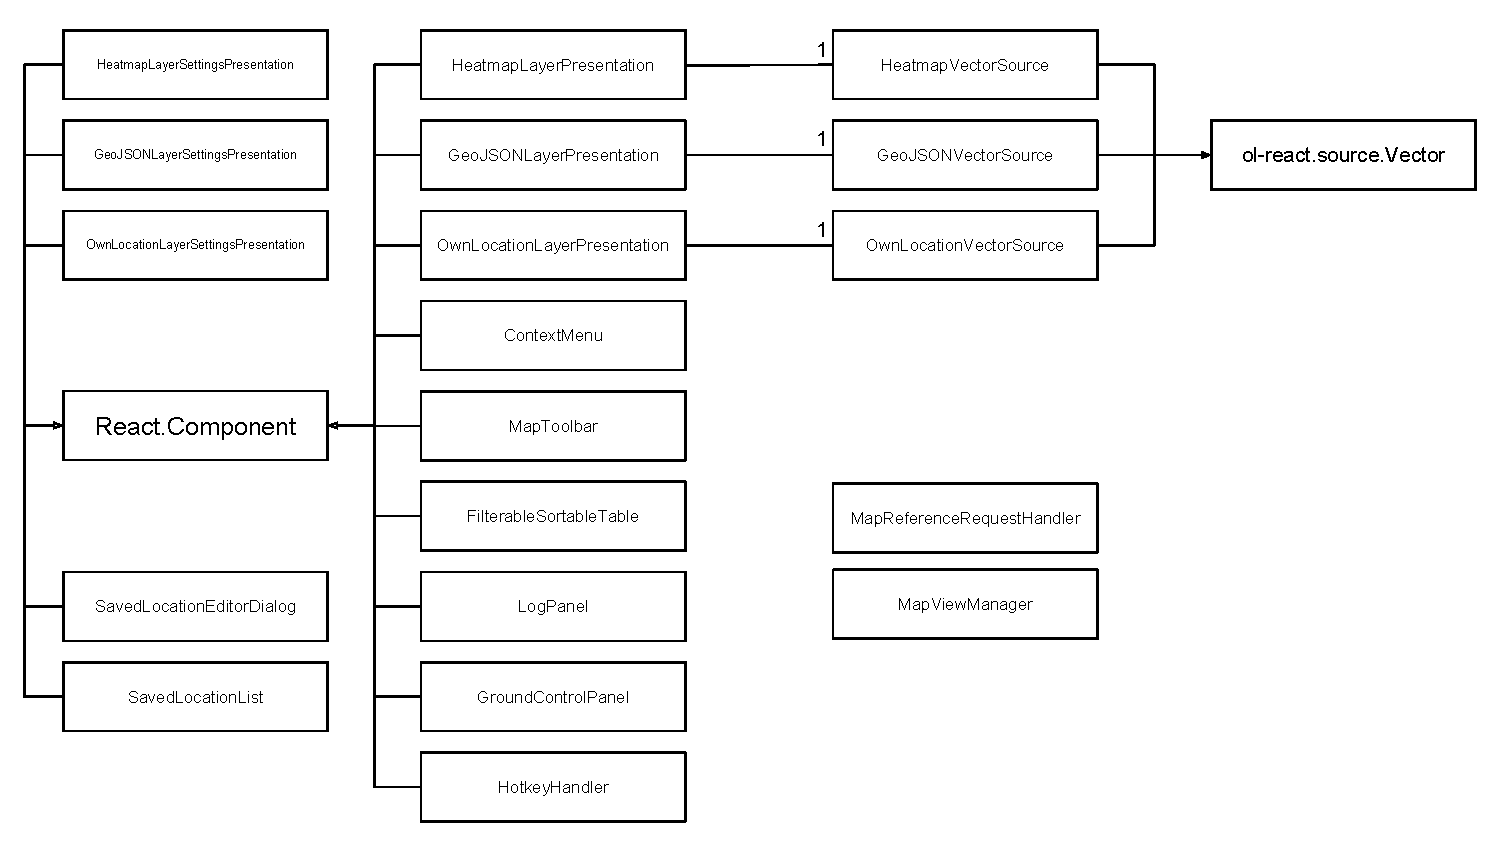
\includegraphics[width=\textwidth]{class_diagram.pdf}
  \caption{Osztálydiagram}
  \label{fig:class_diagram}
\end{figure}
